\section{Architettura}

\subsection{Introduzione}
In questo capitolo verranno descritte brevemente le parti di back-end e di front-end delle 3 webapp.\\
La descrizione dettagliata sarà presente nei capitoli seguenti.\\
\begin{itemize}
    \item \textbf{originIssuer}: originIssuer è la parte front-end della webApp “issuerApp”. Si occupa di comunicare con l’utilizzatore dell’issuerApp, ricevendo i dati in input e restituendo i dati calcolati dal back-end (mediante l’intermediario chiamato Controller). L’interfaccia permette all’utilizzatore di: \begin{itemize}
        \item effettuare il login;
        \item effettuare la registrazione;
        \item permette di vedere le richieste di credenziale da parte degli Account User (soltanto se si effettua il login con l’account Admin);
        \item permette di vedere (tramite una pagina web) la parte di verifica e di validazione delle richieste di credenziale degli account User (soltanto se si effettua il login con l’account Admin);
        \end{itemize}
    \item \textbf{originIssuerApi}: originIssuerApi è la parte back-end della webApp “issuerApp”. Si occupa di calcolare tutti i possibili risultati, che poi verrano poi visualizzati nel front-end della webapp. Il back-end comunica con il controller.Il controller, prima di comunicare con il back-end dopo un input fornito dall’utilizzatore della webApp, effettua alcuni controlli, come per esempio di format (es. se un campo accetta soltanto una variabile numerica, non accetterà altri tipi di variabili e l’operazione si arresta ancor prima di mettere in esecuzione il back-end),alcuni controlli logici,ecc.
    \item \textbf{originVerifier}: originVerifier è la parte front-end della webApp “verifierApp”. Si occupa di comunicare con l’utilizzatore del verifierApp, ricevendo i dati in input e restituendo i dati calcolati dal back-end (mediante l’intermediario chiamato Controller). L’interfaccia permette all’utilizzatore di: \begin{itemize}
        \item effettuare la connessione al proprio wallet (comunicando in questo caso anche con walletApp) per successivamente effettuare l’autenticazione alla piattaforma;
        \item una volta collegato il proprio wallet alla piattaforma, accedere ai servizi offerti da verifierApp;
        \item ci sarà un verificatore (non necessariamente umano, potrebbe essere in alcuni casi anche un controllo automatico) che verifica le richieste di servizi effettuate dall’utente;
        \end{itemize}
    \item \textbf{originVerifierApi}: originVerifierApi è la parte back-end della webApp “verifierApp”. Si occupa di effettuare controlli e di verificare che la credenziale presentata sia valida. Per esempio, il verifier potrebbe controllare che: il documento presentato per accedere al servizio non sia scaduto, che il nome presente nel documento coincida con il nome dell’utente, ecc. In generale, nel back-end si verificano controlli di compatibilità fra i dati scritti nel documento presentato e i dati effettivi che possiede l’utente (data di nascita, luogo di nascita, nome e cognome,ecc.)
    \item \textbf{originWallet}: originWallet è la parte front-end della webApp “walletApp”. L’interfaccia permette all’utilizzatore di: \begin{itemize}
        \item aggiungere i documenti digitali al proprio wallet;
        \item vedere i documenti che sono già conservati all’interno del proprio wallet;
        \item avere una funzionalità (pagina dedicata) per permettere all’utente di cancellare i propri documenti che non desidera più conservare;
        \end{itemize}
    \item \textbf{originWalletApi}: originWalletApi è la parte back-end della webApp “walletApp”. Si occupa di conservare ed organizzare i documenti digitali dell’utente presenti, appunto, nel suo portafoglio digitale (wallet). Quindi si occupa di: \begin{itemize}
        \item conservare i documenti dell’utente;
        \item verificare, mediante dei semplici controlli, di verificare che i documenti siano validi (per esempio, controllando la loro data di scadenza);
        \item cancellare dal wallet i documenti scaduti/non validi;
        \item permettere all’utente in possesso del proprio wallet di cancellare i documenti conservati desiderati;
        \end{itemize}
    \end{itemize}

\subsection{Parte di back-end}
(PARTE MANCANTE, PARTE ROSSA DRIVE)
\subsection{Pattern architetturali e di design}
(INTRODUZIONE ANCORA DA SISTEMARE SU DRIVE)
\begin{itemize}
    \item \textbf{DATA SCRAPPER}: la classe “DataScrapper” contiene delle funzioni per accedere e modificare i dati nel database. DataScrapper è una classe di appoggio e verrà successivamente utilizzata dalla classe DatabaseStrategy.
    Le principali funzioni all'interno di questa classe sono: \begin{itemize}
        \item \textbf{setStrategy(str)}: imposta la strategia di accesso ai dati (Pattern Data Strategy);
        \item \textbf{insertAccount(email, hashed\_pass, salt)}: inserisce un nuovo account nel database con l'indirizzo email, la password hash e il salt fornito;
        \item \textbf{getAccountByEmail(email)}: restituisce un account dal database in base all'indirizzo email ;
        \item \textbf{getAccountById(id)}: restituisce un account dal database in base all'ID fornito;
        \item \textbf{insertSys\_admin(accountId, role)}: inserisce un nuovo sys\_admin (amministratore di sistema) nel database con l'ID dell'account e il ruolo specificato;
        \item \textbf{insertSys\_adminAccount(email, hashed\_pass, salt, role)}: inserisce un nuovo account di amministratore di sistema nel database con l'indirizzo email, la password hash, il salt e il ruolo forniti;
        \item \textbf{getSys\_adminById(id)}: restituisce un amministratore di sistema dal database in base all'ID fornito;
        \item \textbf{insertUser(accountId)}: inserisce un nuovo utente nel database con l'ID dell'account fornito;
        \item \textbf{insertUserAccount(email, hashed\_pass, salt)}: inserisce un nuovo account utente nel database con l'indirizzo email, la password hash e il salt forniti;
        \item \textbf{getUserById(id)}: restituisce un utente dal database in base all'ID fornito;
        \item \textbf{getVCSRequestById(id)}: restituisce una richiesta VCS dal database in base all'ID fornito;
        \item \textbf{getVCSRequestsMarByUserId(id)}: restituisce le richieste VCS di stato civile associate a un utente in base all'ID utente fornito;
        \item \textbf{getVCSRequestMarById(id)}: restituisce una richiesta VCS di stato civile dal database in base all'ID fornito;
        \item \textbf{insertVCSRequestMar(applicantId, status, personalIdentifier)}: inserisce una nuova richiesta VCS di stato civile nel database con l'ID dell'applicante, lo stato e l'identificatore personale forniti;
        \item \textbf{getVCSRequestsPidByUserId(id)}: restituisce le richieste VCS PID (Personal Identifier) associate a un utente in base all'ID utente fornito;
        \item \textbf{getVCSRequestPidById(id)}: restituisce una richiesta VCS PID dal database in base all'ID fornito;
        \item \textbf{insertVCSRequestPid(applicantId, currentAddress, dateOfBirth, familyName, firstName, gender, nameAndFamilyNameAtBirth, personalIdentifier, placeOfBirth)}: inserisce una nuova richiesta VCS PID nel database con i dettagli specificati;
        \item \textbf{getVCSRequestVerification(id)}: restituisce una verifica della richiesta VCS dal database in base all'ID fornito;
        \item \textbf{updateVCSRequestReleased(vcs\_requestId, released)}: aggiorna lo stato di rilascio di una richiesta VCS specificata nel database;
        \item \textbf{updateVCSRequestVerificationStatus(vcs\_requestId, status)}: aggiorna lo stato di verifica di una richiesta VCS specificata nel database;
        \item \textbf{getVCSRequestsPending()}: restituisce le richieste VCS con lo stato “in sospeso” dal database;
        \item \textbf{getVCSRequestsNotPending()}: restituisce le richieste VCS non “in sospeso” dal database;
        \item \textbf{insertVCSRequestVerification(vcs\_request, admin\_verifier, status)}: inserisce una nuova verifica di richiesta VCS nel database con i dettagli specificati.
        \end{itemize}
    
    \item \textbf{DATABASE STRATEGY}: (ASPETTO CONFERMA SE POSSO STENDERE)
    \item \textbf{ROUTING}: (DA SISTEMARE)
    \end{itemize}
\subsubsection{Database}\label{Database}

\paragraph{Introduzione}
Tenendo conto dei requisiti e dell’archittettura da rispettare del capitolato, si sono sviluppati 2 database: “issuerdb” per l’Issuer e “walletdb”  per lo User (cioè l’utente in possesso del proprio portafoglio digitale).

\paragraph{Issuerdb}
    
\begin{center}
    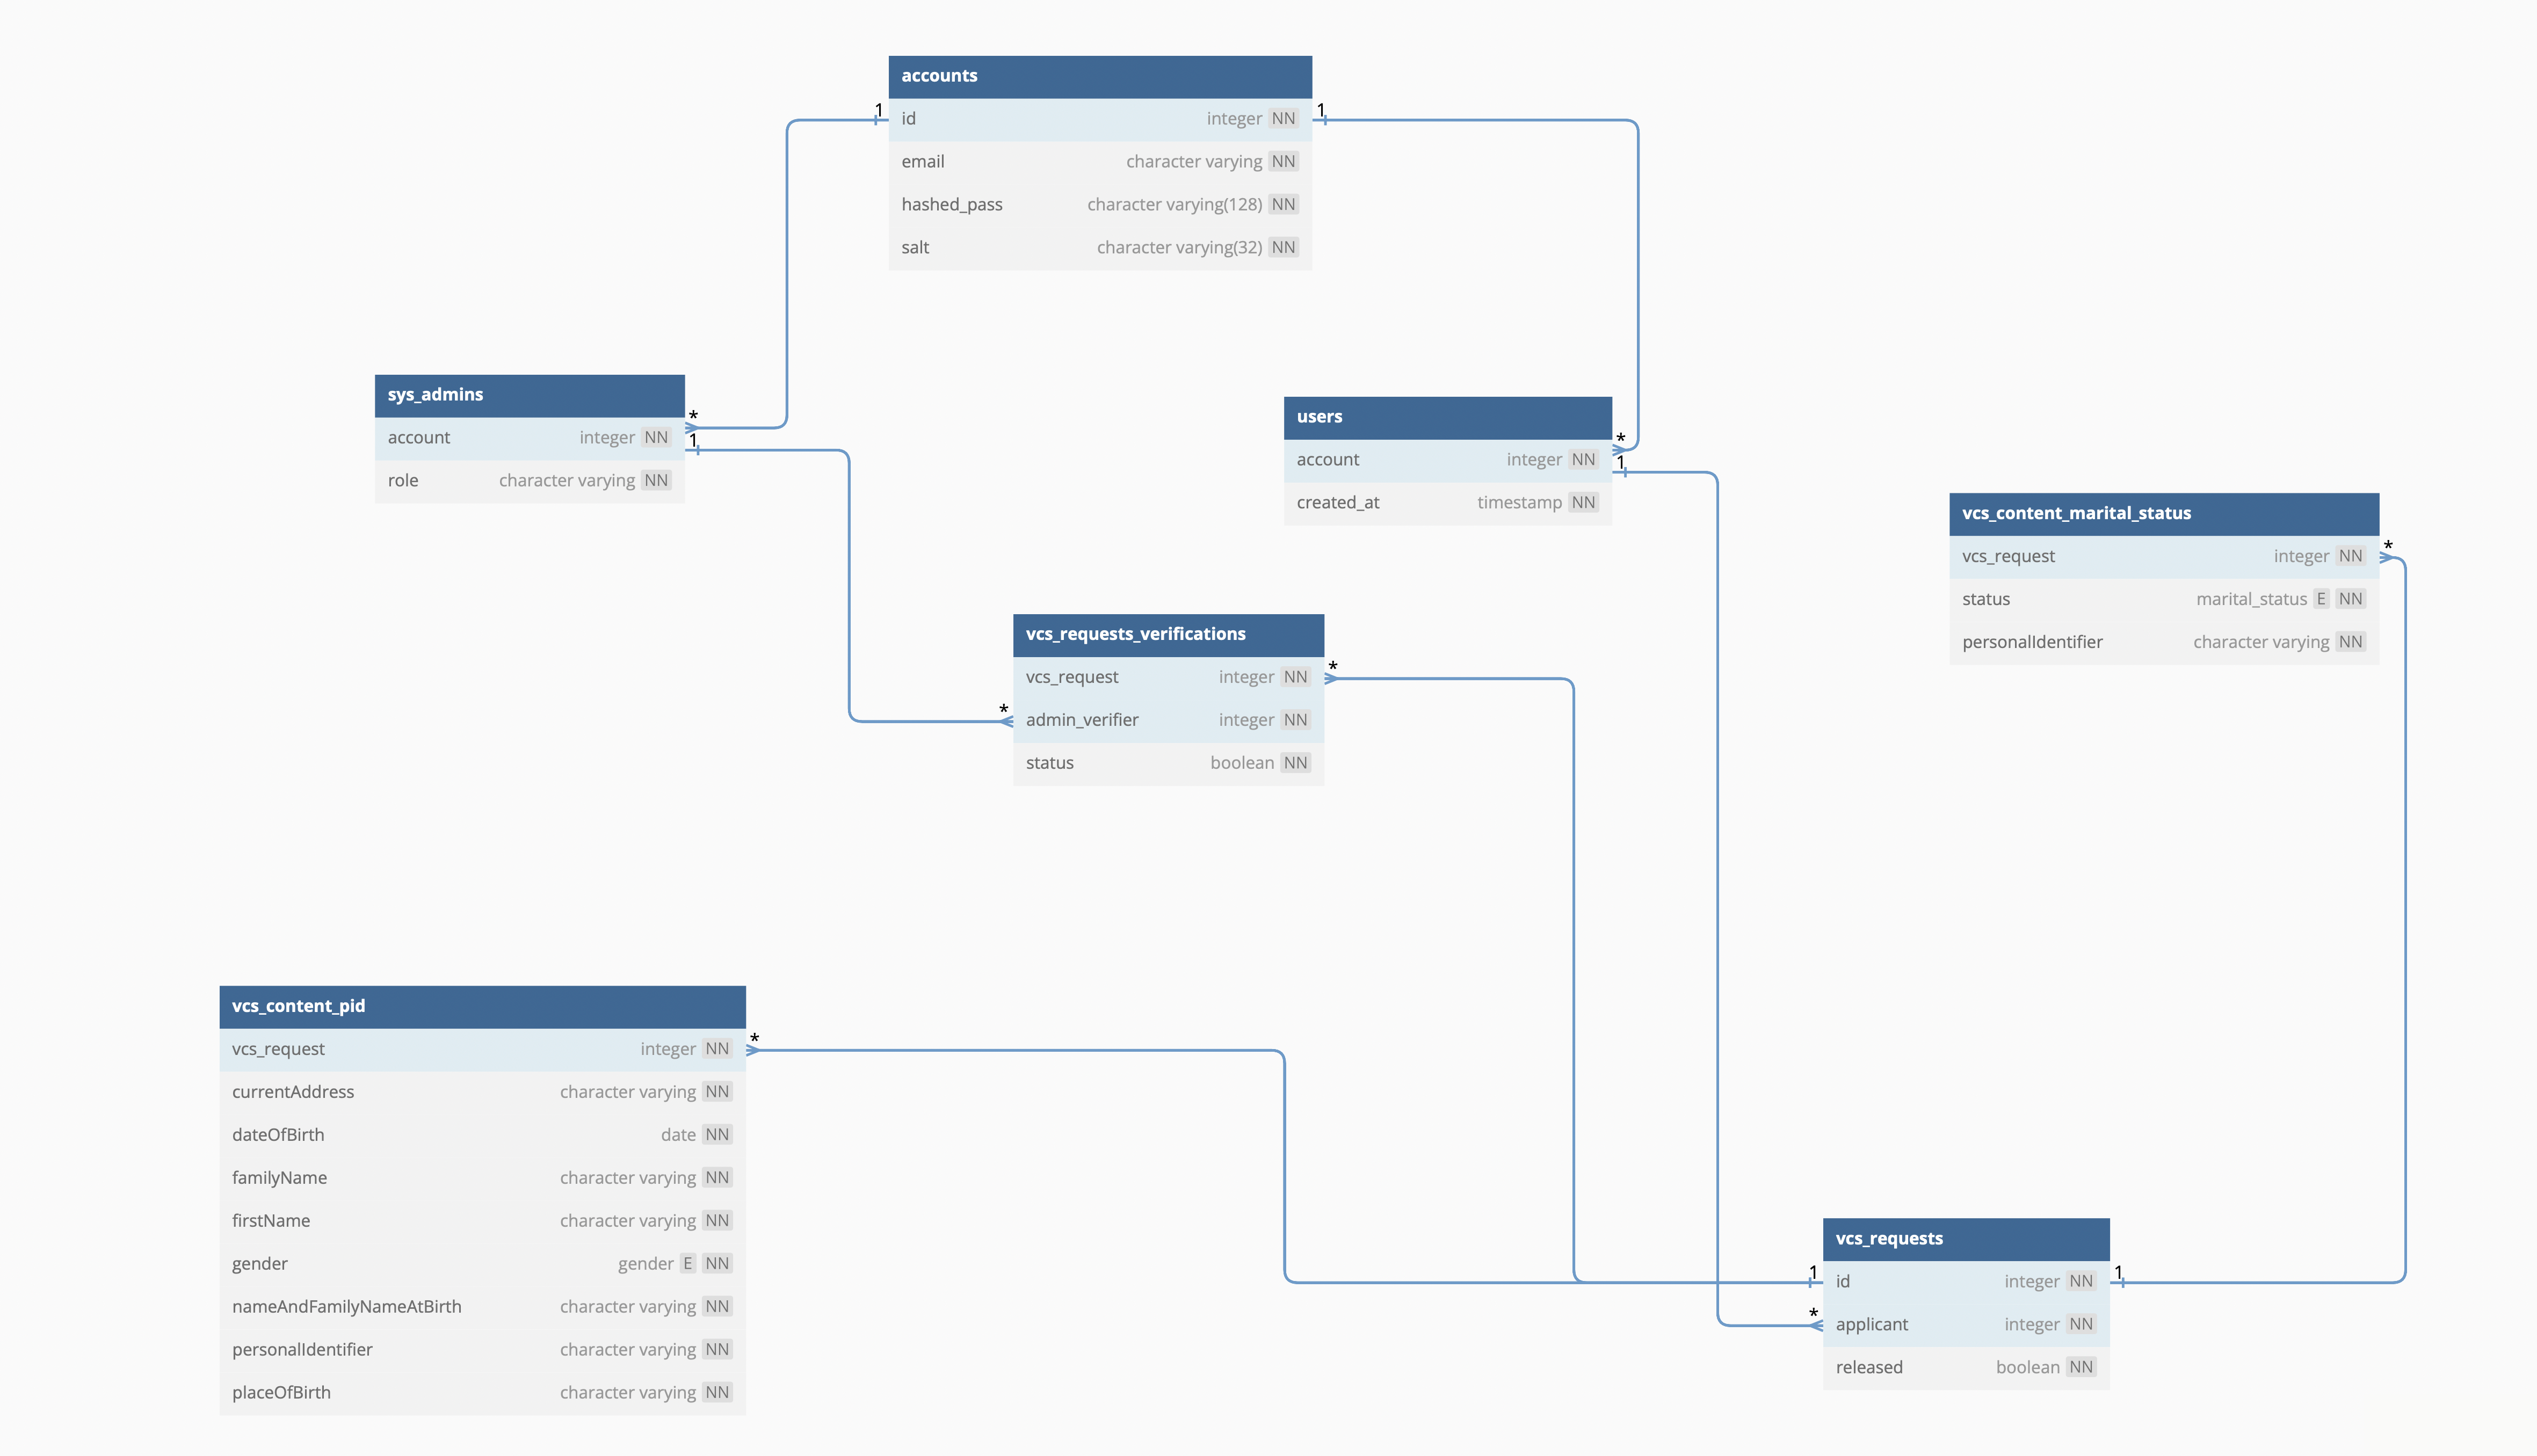
\includegraphics[scale = 0.9]{./res/img/issuerdb.png}
  \end{center}
L'immagine sopra riportata descrive il database "issuerdb" implementato mediante un grafico entità-relazioni (schema ER).\\
Issuerdb è stato pensato per gestire e conservare le informazioni legate agli utenti, alle richieste di certificati digitali (VCS requests) e alle verifiche dei certificati stessi.
Per quanto richiesto dal capitolato, e per rispettare la logica dietro tutto il meccanismo dell'Issuer, si distinguono 2 tipi diversi di account: gli account "sys\_admins" e gli account "users".\\
\begin{itemize}
\item "sys\_admins" sono gli account utilizzati dagli amministratori di sistema, cioè quelle entità che si occupano di approvare (o meglio, verificare) le richieste degli "users" (VCS requests).\\
\item "users", invece, sono gli account utilizzati dai semplici utilizzatori del servizio. Si occupano semplicemente di effettuare delle richieste di certificati di loro interesse alle entità che si occupano di verificare i certificati.\\
\end{itemize}
Il contenuto della richiesta approvata e rilasciata può essere di 2 tipi soltanto: un "vcs\_content\_marital\_status" (contenuto riferito allo stato di matrimonio di un utente) o un "vcs\_content\_pid" (contenuto riferito ad un documento PID di un utente).\\
Più in dettaglio:\\\\
\textbf{Tipi enumerati}: sono definite due tabelle ENUM per rappresentare:
\begin{itemize}
    \item il genere maschile/femminile (“gender”, che può avere come valori “M” o “F”);
    \item lo stato civile (“marital\_status”, che può avere come valori “married”, “cohabitant”, “divorced”,”widower”, “separate”, “canceled”, “other”).
\end{itemize}
Queste tabelle verranno utilizzate per definire, rispettivamente, gli attributi “gender” della tabella “vcs\_content\_pid” e “marital\_status” della tabella “vcs\_content\_marital\_status”.\\\\

\textbf{Tabella “accounts”}:
\begin{itemize}
    \item “id”: identificativo univoco per l’account, chiave primaria; 
    \item “email”: indirizzo email dell’account, varchar not null;
    \item “hashed\_pass”: password hash dell’account, varchar massimo 60 caratteri not null;
    \item “salt”: salt usato per la sicurezza nella creazione dell’hash della password dell’account dell’utente, varchar massimo 22 caratteri not null.
\end{itemize}

\textbf{Tabella “users”}:
\begin{itemize}
    \item “account”: riferimento all'id della tabella "accounts", identificativo univoco per l’account degli utilizzatori,  chiave primaria;
    \item “created\_at”: data di creazione dell’account, formato timestamp not null. 
\end{itemize}

\textbf{Tabella “sys\_admins”}:
\begin{itemize}
    \item “account”: riferimento all'id della tabella "accounts", identificativo univoco per l’account degli amministratori,  chiave primaria; 
    \item “role”: ruolo dell'amministratore di sistema, varchar not null.
\end{itemize}

\textbf{Tabella “vcs\_requests”}:
\begin{itemize}
    \item “id”: identificativo univoco della richiesta del certificato; 
    \item “applicant”: riferimento all'account dell'utente nella tabella "users", integer not null;  
    \item “released”: flag per indicare se il certificato è stato rilasciato, variabile booleana not null. 
\end{itemize}

\textbf{Tabella “vcs\_requests\_verifications”}:
\begin{itemize}
    \item “vcs\_request”: riferimento all'id di una richiesta nella tabella "vcs\_requests";  
    \item “admin\_verifier”: riferimento all'account dell'amministratore di sistema;  
    \item “status”: stato della verifica, variabile booleana not null. 
\end{itemize}

\textbf{Tabella “vcs\_content\_pid”}:
\begin{itemize}
    \item “vcs\_request”: riferimento all'identificativo di una richiesta nella tabella "vcs\_requests" e “vcs\_requests\_verifications”; 
    \item “currentAddress”: l’indirizzo corrente scritto nel documento PID, varchar not null; 
    \item “dateOfBirth”: data di nascita scritta nel documento PID, varchar not null;  
    \item “familyName”: cognome scritto nel documento PID, varchar not null; 
    \item “firstName”: nome scritto nel documento PID, varchar not null; 
    \item “gender”: genere scritto nel documento PID, enum con valori “M”/”F” not null; 
    \item “identifier”: identificatore scritto nel documento PID, varchar not null; 
    \item “nameAndFamilyNameAtBirth”: nome e cognome di famiglia scritto nel documento PID, varchar not null;
    \item “personalIdentifier”: identificatore personale scritto nel documento PID, varchar not null.
\end{itemize}

\textbf{Tabella “vcs\_content\_marital\_status”}:
\begin{itemize}
    \item “vcs\_request”: riferimento all'identificativo di una richiesta nella tabella "vcs\_requests" e “vcs\_requests\_verifications”; 
    \item “status”: stato civile = stato di matrimonio, enum corrispondente ai valori della tabella “marital\_status”, not null;  
    \item “personalIdentifier”: identificatore personale per es. codice fiscale, varchar not null.
\end{itemize}


\textbf{RELAZIONI FRA LE TABELLE}
\begin{itemize}
    \item \textbf{“accounts” – “sys\_admins” e “users”}: “accounts” – “sys\_admins” e “accounts” – “users” relazione 1-1. Un account appartiene a un solo utente, un utente può avere soltanto un account. Un account appartiene a un solo amministratore, un amministratore può avere solo un account. Un account è un account “sys\_admins” oppure un account “users”, non può essere entrambi. La relazione deve essere unica, e questo limite si controlla nel back-end (poiché nel database non c’è modo di controllare l’unicità della relazione). Nel back-end si controllerà anche se un account è sia un account amministratore che un account user (con conseguente errore).
    \item \textbf{“sys\_admins” – “vcs\_requests\_verifications”}: relazione 1-N. Una verifica di richiesta appartiene al massimo ad un amministratore. Un amministratore può verificare molteplici richieste.
    \item \textbf{“users” – “vcs\_requests”}: relazione 1-N. Una richiesta di credenziale può appartenere al massimo ad un user. Un user può fare molteplici richieste.
    \item \textbf{“vcs\_requests\_verifications” e “vcs\_requests” – “vcs\_content\_marital\_status” e “vcs\_content\_pid”}: similmente a prima, il contenuto del VCS o è un contenuto relativo al “marital status”, oppure un contenuto relativo al “PID” (non entrambi, ma deve essere obbligatoriamente un contenuto di marital status oppure un contenuto di PID). Questa condizione sarà controllata nel back-end. La richiesta sarà rilasciata DOPO che la richiesta sarà approvata dal verificatore. Per essere rilasciata (dopo essere approvata), l’utente riceve la richiesta come credenziale (con conseguente stoccaggio nel “walletdb”). Una volta ricevuta, la richiesta verrà contrassegnata come “true” (nel campo “released” in “vcs\_requests”). Invece, il campo “status” in “vcs\_requests\_verifications” indica se la richiesta è stata approvata dal verificatore. Se lo “status” sarà “true”, allora la richiesta sarà pronta per il rilascio (quindi lo status “true” dell’attributo “released” di “vcs\_requests” dipende dallo status “true” dell’attributo “status” di “vcs\_requests\_verifications”). Una richiesta può essere verificata una sola volta. Una verifica appartiene ad una e una sola richiesta. Se la richiesta non è stata ancora approvata non si può richiedere una riapprovazione. Se la richiesta è stata verificata con esito status=”false” soltanto allora si può fare un altro tentativo di richiesta. Per questo motivo la relazione fra “vcs\_requests” e “vcs\_requests\_verifications” è 1-1.
\end{itemize}



\paragraph{Walletdb}
\begin{center}
    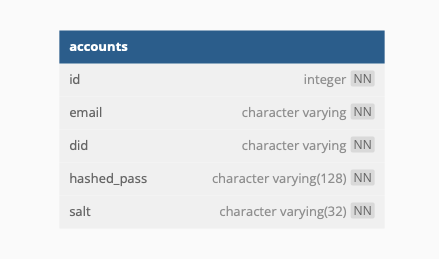
\includegraphics[scale = 0.3]{./res/img/walletdb.png}
  \end{center}

L’immagine sopra riportata descrive il database “walletdb” implementato mediante un grafico entità-relazioni (schema ER).
Walletdb è stato pensato per gestire e conservare (fare lo “storing”) le informazioni legate alle credenziali degli utenti, come espresso da capitolato.\\
Più in dettaglio:\\\\
\textbf{Tabella “accounts”}:
\begin{itemize}
    \item "id": identificativo univoco per l'account degli utenti, chiave primaria,
    \item "email": indirizzo email associato all'account, varchar not null,
    \item "did": documento did associato all'account dell'utente, varchar,
    \item "hashed\_pass": password hash dell'account dell'utente, varchar massimo 60 caratteri not null,
    \item "salt": salt usato per la sicurezza nella creazione dell'hash della password dell'account dell'utente, varchar massimo 22 caratteri not null,
    \item “created\_at”: data di creazione dell’account, timestamp not null.
\end{itemize}

\subsection{Parte di front-end}
(PARTE MANCANTE, PARTE ROSSA DRIVE)
\subsubsection{React Material-UI}
Material-UI è una libreria di componenti UI (User Interface) per React fatto da Google. Material-UI è una libreria che viene utilizzata principalmente per realizzare interfacce utente dinamiche e personalizzate.
Segue il design system “Material Design”, che si occupa di fornire linee guida di design per la realizzazione di applicazioni e siti web.
Alcune caratteristiche che sono state di gradimento per la scelta di questa libreria all’interno del progetto Personal Identity Wallet sono state:
\begin{itemize}
    \item la libreria offre una vasta gamma di componenti UI predefiniti (pre-implementati). Questo permette di facilitare lo sviluppo dell’interfaccia grafica, con un notevole accorciamento delle tempistiche;
    \item i componenti sono inoltre facilmente personalizzabili, il ché permette di integrarsi facilmente all’interno del progetto e di soddisfare i requisiti imposti dal capitolato;
    \item è una libreria ben documentata: in caso di dubbi si può consultare la documentazione ufficiale. Inoltre nella community si possono trovare numerosi esempi pratici per ottenere familiarità (oppure cercare risposte ai vari problemi di implementazione) con Material-UI;
    \item è stata realizzata specificamente per React. Questo significa che si integra perfettamente con il framework;
    \item inoltre, è compatibile con una buona parte delle altre librerie di React;
\end{itemize}
\subsection{Componente di API}


\subsection{Design pattern}